%%%%%%%%%%%%%%%%%%%%%%%%%%%%%%%%%%%%%%%%%%%%%%%%%%%%%%%%%%%%%%%
%% OXFORD THESIS TEMPLATE

% Use this template to produce a standard thesis that meets the Oxford University requirements for DPhil submission
%
% Originally by Keith A. Gillow (gillow@maths.ox.ac.uk), 1997
% Modified by Sam Evans (sam@samuelevansresearch.org), 2007
% Modified by John McManigle (john@oxfordechoes.com), 2015
% Modified by Ulrik Lyngs (ulrik.lyngs@cs.ox.ac.uk), 2018, for use with R Markdown
%
% Ulrik Lyngs, 25 Nov 2018: Following John McManigle, broad permissions are granted to use, modify, and distribute this software
% as specified in the MIT License included in this distribution's LICENSE file.
%
% John tried to comment this file extensively, so read through it to see how to use the various options.  Remember
% that in LaTeX, any line starting with a % is NOT executed.  Several places below, you have a choice of which line to use
% out of multiple options (eg draft vs final, for PDF vs for binding, etc.)  When you pick one, add a % to the beginning of
% the lines you don't want.


%%%%% CHOOSE PAGE LAYOUT
% The most common choices should be below.  You can also do other things, like replacing "a4paper" with "letterpaper", etc.

% This one will format for two-sided binding (ie left and right pages have mirror margins; blank pages inserted where needed):
%\documentclass[a4paper,twoside]{templates/ociamthesis}
% This one will format for one-sided binding (ie left margin > right margin; no extra blank pages):
%\documentclass[a4paper]{ociamthesis}
% This one will format for PDF output (ie equal margins, no extra blank pages):
%\documentclass[a4paper,nobind]{templates/ociamthesis}
%UL 2 Dec 2018: pass this in from YAML
\documentclass[a4paper, twoside]{templates/ociamthesis}

% UL 5 January 2021 - add packages used by kableExtra
\usepackage{booktabs}
\usepackage{longtable}
\usepackage{array}
\usepackage{multirow}
\usepackage{wrapfig}
\usepackage{colortbl}
\usepackage{pdflscape}
\usepackage{tabu}
\usepackage{threeparttable}
\usepackage{threeparttablex}
\usepackage[normalem]{ulem}
\usepackage{makecell}
\usepackage[colorlinks=false,pdfpagelabels,hidelinks=true]{hyperref}
\usepackage{float}


%UL set section header spacing
\usepackage{titlesec}
% 
\titlespacing\subsubsection{0pt}{24pt plus 4pt minus 2pt}{0pt plus 2pt minus 2pt}

% UL 30 Nov 2018 pandoc puts lists in 'tightlist' command when no space between bullet points in Rmd file
\providecommand{\tightlist}{%
  \setlength{\itemsep}{0pt}\setlength{\parskip}{0pt}}
 
% UL 1 Dec 2018, fix to include code in shaded environments

%UL set whitespace around verbatim environments
\usepackage{etoolbox}
\makeatletter
\preto{\@verbatim}{\topsep=0pt \partopsep=0pt }
\makeatother

%UL 26 Mar 2019, enable strikethrough
\usepackage[normalem]{ulem}

%UL use soul package for correction highlighting
\usepackage{color, soul}
\usepackage{xcolor}
\definecolor{correctioncolor}{HTML}{CCCCFF}
\sethlcolor{correctioncolor}
\newcommand{\ctext}[3][RGB]{%
  \begingroup
  \definecolor{hlcolor}{#1}{#2}\sethlcolor{hlcolor}%
  \hl{#3}%
  \endgroup
}
\soulregister\ref7
\soulregister\cite7
\soulregister\autocite7
\soulregister\textcite7
\soulregister\pageref7

%%%%%%% PAGE HEADERS AND FOOTERS %%%%%%%%%
\usepackage{fancyhdr}
\setlength{\headheight}{15pt}
\fancyhf{} % clear the header and footers
\pagestyle{fancy}
\renewcommand{\chaptermark}[1]{\markboth{\thechapter. #1}{\thechapter. #1}}
\renewcommand{\sectionmark}[1]{\markright{\thesection. #1}} 
\renewcommand{\headrulewidth}{0pt}

\fancyhead[LO]{\emph{\leftmark}} 
\fancyhead[RE]{\emph{\rightmark}} 

% UL page number position 
\fancyfoot[C]{\emph{\thepage}} %regular pages
\fancypagestyle{plain}{\fancyhf{}\fancyfoot[C]{\emph{\thepage}}} %chapter pages

% JEM fix header on cleared pages for openright
\def\cleardoublepage{\clearpage\if@twoside \ifodd\c@page\else
   \hbox{}
   \fancyfoot[C]{}
   \newpage
   \if@twocolumn\hbox{}\newpage
   \fi
   \fancyhead[LO]{\emph{\leftmark}} 
   \fancyhead[RE]{\emph{\rightmark}} 
   \fi\fi}


%%%%% SELECT YOUR DRAFT OPTIONS
% This adds a "DRAFT" footer to every normal page.  (The first page of each chapter is not a "normal" page.)

% This highlights (in blue) corrections marked with (for words) \mccorrect{blah} or (for whole
% paragraphs) \begin{mccorrection} . . . \end{mccorrection}.  This can be useful for sending a PDF of
% your corrected thesis to your examiners for review.  Turn it off, and the blue disappears.

% IP feb 2021: option to include line numbers in PDF
\usepackage{lineno}
\linenumbers

%%%%% BIBLIOGRAPHY SETUP
% Note that your bibliography will require some tweaking depending on your department, preferred format, etc.
% If you've not used LaTeX before, I recommend reading a little about biblatex/biber and getting started with it.
% If you're already a LaTeX pro and are used to natbib or something, modify as necessary.
% Either way, you'll have to choose and configure an appropriate bibliography format...


\usepackage[style=authoryear, sorting=nyt, backend=biber, maxcitenames=2, useprefix, doi=true, isbn=false, uniquename=false]{biblatex}
\newcommand*{\bibtitle}{Works Cited}

\addbibresource{references.bib}


% This makes the bibliography left-aligned (not 'justified') and slightly smaller font.
\renewcommand*{\bibfont}{\raggedright\small}


% Uncomment this if you want equation numbers per section (2.3.12), instead of per chapter (2.18):
%\numberwithin{equation}{subsection}


%%%%% THESIS / TITLE PAGE INFORMATION
% Everybody needs to complete the following:
\title{Thesis title}
\author{Faes E.\footnote{\href{mailto:Enjo.Faes@student.ams.ac.be}{\nolinkurl{Enjo.Faes@student.ams.ac.be}}}\textsuperscript{}~~~Mertens de Wilmars S.\footnote{\href{mailto:Stephane.MertensdeWilmars@student.ams.ac.be}{\nolinkurl{Stephane.MertensdeWilmars@student.ams.ac.be}}}\textsuperscript{}~~~Pratesi F.\footnote{\href{mailto:Filippo.Pratesi@student.ams.ac.be}{\nolinkurl{Filippo.Pratesi@student.ams.ac.be}}}\textsuperscript{}}
\college{}

% Master's candidates who require the alternate title page (with candidate number and word count)
% must also un-comment and complete the following three lines:

% Uncomment the following line if your degree also includes exams (eg most masters):
%\renewcommand{\submittedtext}{Submitted in partial completion of the}
% Your full degree name.  (But remember that DPhils aren't "in" anything.  They're just DPhils.)
\degree{Master in Finance}
% Term and year of submission, or date if your board requires (eg most masters)
\degreedate{June 2021}


%%%%% YOUR OWN PERSONAL MACROS
% This is a good place to dump your own LaTeX macros as they come up.

% To make text superscripts shortcuts
	\renewcommand{\th}{\textsuperscript{th}} % ex: I won 4\th place
	\newcommand{\nd}{\textsuperscript{nd}}
	\renewcommand{\st}{\textsuperscript{st}}
	\newcommand{\rd}{\textsuperscript{rd}}

%%%%% THE ACTUAL DOCUMENT STARTS HERE
\begin{document}

%%%%% CHOOSE YOUR LINE SPACING HERE
% This is the official option.  Use it for your submission copy and library copy:
\setlength{\textbaselineskip}{22pt plus2pt}
% This is closer spacing (about 1.5-spaced) that you might prefer for your personal copies:
%\setlength{\textbaselineskip}{18pt plus2pt minus1pt}

% You can set the spacing here for the roman-numbered pages (acknowledgements, table of contents, etc.)
\setlength{\frontmatterbaselineskip}{17pt plus1pt minus1pt}

% UL: You can set the line and paragraph spacing here for the separate abstract page to be handed in to Examination schools
\setlength{\abstractseparatelineskip}{13pt plus1pt minus1pt}
\setlength{\abstractseparateparskip}{0pt plus 1pt}

% UL: You can set the general paragraph spacing here - I've set it to 2pt (was 0) so
% it's less claustrophobic
\setlength{\parskip}{2pt plus 1pt}

%
% Oxford University logo on title page
%
\def\crest{{
\includegraphics{templates/amslogo.pdf}}}
\renewcommand{\university}{Antwerp Management School}
\renewcommand{\submittedtext}{A thesis submitted for the degree of}
\renewcommand{\submittedtext}{Prof.~dr. Annaert ~Prof.~dr. De Ceuster ~Prof.~dr. Zhang}


% Leave this line alone; it gets things started for the real document.
\setlength{\baselineskip}{\textbaselineskip}


%%%%% CHOOSE YOUR SECTION NUMBERING DEPTH HERE
% You have two choices.  First, how far down are sections numbered?  (Below that, they're named but
% don't get numbers.)  Second, what level of section appears in the table of contents?  These don't have
% to match: you can have numbered sections that don't show up in the ToC, or unnumbered sections that
% do.  Throughout, 0 = chapter; 1 = section; 2 = subsection; 3 = subsubsection, 4 = paragraph...

% The level that gets a number:
\setcounter{secnumdepth}{2}
% The level that shows up in the ToC:
\setcounter{tocdepth}{2}


%%%%% ABSTRACT SEPARATE
% This is used to create the separate, one-page abstract that you are required to hand into the Exam
% Schools.  You can comment it out to generate a PDF for printing or whatnot.

% JEM: Pages are roman numbered from here, though page numbers are invisible until ToC.  This is in
% keeping with most typesetting conventions.
\begin{romanpages}

% Title page is created here
\maketitle

%%%%% DEDICATION -- If you'd like one, un-comment the following.
\begin{dedication}
  For Yihui Xie
\end{dedication}

%%%%% ACKNOWLEDGEMENTS -- Nothing to do here except comment out if you don't want it.
\begin{acknowledgements}
 	First of all, many thanks to our families and loved ones that supported us during the writing of this thesis. Secondly, thank you professors \href{https://www.antwerpmanagementschool.be/nl/faculty/hairui-zhang}{Zhang}, \href{https://www.antwerpmanagementschool.be/nl/faculty/jan-annaert}{Annaert} and \href{https://www.antwerpmanagementschool.be/nl/faculty/marc-de-ceuster}{De Ceuster} for the valuable insights you have given us in preparation of this thesis and the many questions answered. We must be grateful for the classes of R programming by prof Zhang. ~\\

  \noindent Secondly, we have to thank the developer of the software we used for our thesis. A profuse thanks to Allaire, the founder and CEO of \href{http://rstudio.com}{RStudio}. Thanks for making data science easier, more accessible and fun. We must also be grateful to Gruber for inventing ``Markdown'', to MacFarlane for creating ``Pandoc'' which converts Markdown to a large number of output formats, and to Xie for creating ``knitr'' which introduced R Markdown as a way of embedding code in Markdown documents, and ``bookdown'' which added tools for technical and longer-form writing.Special thanks to \href{http://chester.rbind.io}{Ismay}, who created the ``thesisdown'' package that helped many PhD students write their theses in R Markdown. And a very special thanks to McManigle, whose adaption of Evans' adaptation of Gillow's original maths template for writing an Oxford University DPhil thesis in ``LaTeX'' provided the template that Ulrik Lyngs in turn adapted for R Markdown, which we also owe a big thank you. Without which this thesis could not have been written in this format \autocite{lyngsOxforddown2019}. ~\\

  \noindent Finally, we thank \textcite{alexios2020} for making the implementation of GARCH models integrated in R via his package ``Rugarch''. By doing this, he facilitated the process of understanding the whole process and doing the analysis for our thesis. ~\\

  \begin{flushright}
  Enjo Faes, \\
  Stephane Mertens de Wilmars, \\
  Filippo Pratesi \\
  Antwerp Management School, Antwerp \\
  27 June 2021
  \end{flushright}
\end{acknowledgements}


%%%%% ABSTRACT -- Nothing to do here except comment out if you don't want it.
\begin{abstract}
	The greatest abstract all times
\end{abstract}

%%%%% MINI TABLES
% This lays the groundwork for per-chapter, mini tables of contents.  Comment the following line
% (and remove \minitoc from the chapter files) if you don't want this.  Un-comment either of the
% next two lines if you want a per-chapter list of figures or tables.

% This aligns the bottom of the text of each page.  It generally makes things look better.
\flushbottom

% This is where the whole-document ToC appears:
\tableofcontents

\listoffigures
	\mtcaddchapter
  	% \mtcaddchapter is needed when adding a non-chapter (but chapter-like) entity to avoid confusing minitoc

% Uncomment to generate a list of tables:
\listoftables
  \mtcaddchapter
%%%%% LIST OF ABBREVIATIONS
% This example includes a list of abbreviations.  Look at text/abbreviations.tex to see how that file is
% formatted.  The template can handle any kind of list though, so this might be a good place for a
% glossary, etc.
% First parameter can be changed eg to "Glossary" or something.
% Second parameter is the max length of bold terms.
\begin{mclistof}{List of Abbreviations}{3.2cm}
\item[ACD] Autoregressive Conditional Density models (Hansen, 1994)
\item[ARCH] Autoregressive Conditional Heteroscedasticity model (Bollerslev, 1986)
\item[GARCH] Generalized Autoregressive Conditional Heteroscedasticity model (Bollerslev, 1986)
\item[IGARCH] Integrated GARCH (Bollerslev, 1986)
\item[EGARCH] Exponential GARCH (Nelson, 1991)
\item[GJRGARCH] Glosten-Jagannathan-Runkle GARCH model (Glosten et al. 1993)
\item[NAGARCH] Nonlinear asymmetric GARCH (Engle and Ng, 1993)
\item[TGARCH] Threshold GARCH (Zakoian, 1994)
\item[TSGARCH] Also called Absolute Value GARCH or AVGARCH referring to Taylor (1986) and Schwert (1989)
\item[EWMA] Exponentially Weighted Moving Average model 
\item[i.i.d, iid] Independent and identically distributed
\item[T] Student's T-distribution
\item[ST] Skewed Student's T-distribution
\item[SGT] Skewed Generalized T-distribution
\item[GED] Generalized Error Distribution
\item[SGED] Skewed Generalized Error Distribution
\item[NORM] Normal distribution
\item[VaR] Value-at-Risk 
\item[cVaR] Expected shortfall or conditional Value-at-Risk
\end{mclistof} 


% The Roman pages, like the Roman Empire, must come to its inevitable close.
\end{romanpages}

%%%%% CHAPTERS
% Add or remove any chapters you'd like here, by file name (excluding '.tex'):
\flushbottom

% all your chapters and appendices will appear here
\hypertarget{introduction}{%
\chapter*{Introduction}\label{introduction}}
\addcontentsline{toc}{chapter}{Introduction}

\adjustmtc
\markboth{Introduction}{}

A general assumption in finance is that stock returns are normally distributed (\ldots). However, various authors have shown that this assumption does not hold in practice: stock returns are not normally distributed (\ldots). For example, \textcite{theodossiou2000} mentions that ``empirical distributions of log-returns of several financial assets exhibit strong higher-order moment dependencies which exist mainly in daily and weekly log-returns and prevent monthly, bimonthly and quarterly log-returns from obeying the normality law implied by the central limit theorem. As a consequence, price changes do not follow the geometric Brownian motion.'' So in reality, stock returns exhibit fat-tails and peakedness (\ldots), these are some of the so-called stylized facts of returns.

Additionally a point of interest is the predictability of stock prices. \textcite{fama1965} explains that the question in academic and business circles is: ``To what extent can the past history of a common stock's price be used to make meaningful predictions concerning the future price of the stock?''. There are two viewpoints towards the predictability of stock prices. Firstly, some argue that stock prices are unpredictable or very difficult to predict by its past returns (i.e.~have very little serial correlation) because they simply follow a Random Walk process (\ldots). On the other hand, Lo \& MacKinlay mention that ``financial markets \emph{are} predictable to some extent but far from being a symptom of inefficiency or irrationality, predictability is the oil that lubricates the gears of capitalism''. Furthermore, there is also no real robust evidence for the predictability of returns themselves, let alone be out-of-sample \autocite{welch2008}. This makes it difficult for corporations to manage market risk, i.e.~the variability of stock prices.

Risk in general can be defined as the volatility of unexpected outcomes \autocite{jorion2007}. The measure Value at Risk (VaR), developed in response to the financial disaster events of the early 1990s, has been very important in the financial world. Corporations have to manage their risks and thereby include a future risk measurement.

\hypertarget{lit-rev}{%
\chapter{Literature review}\label{lit-rev}}

\minitoc 

\hypertarget{stylized-facts-of-returns}{%
\section{Stylized facts of returns}\label{stylized-facts-of-returns}}

When analyzing returns as a time-series, we look at log returns. The log returns are similar to simple returns so the stylized facts of returns apply to both. One assumption that is made often in financial applications is that returns are iid, or independently and identically distributed, another is that they are normally distribution. Are these valid assumptions? Below the stylized facts\footnote{Stylized facts are the statistical properties that appear to be present in many empirical asset returns (across time and markets)} following \textcite{annaert2021} for returns are given.

\begin{itemize}
\item
  Returns are \emph{small and volatile} (with the standard deviation being larger than the mean on average)
\item
  Returns have very little serial correlation as mentioned by for example \textcite{bollerslev1987}.
\item
  Returns exhibit conditional heteroskedasticity, or \emph{volatility clustering}. There is no constant variance, but it is time-varying (homoskedasticity). \textcite{bollerslev1987} describes it as ``rates of return data are characterized by volatile and tranquil periods''.
\item
  Returns also exhibit \emph{asymmetric volatility}, in that sense volatility increases more after a negative return shock than after a large positive return shock. This is also called the \emph{leverage effect.}
\item
  Returns are \emph{not normally distributed} which is also one of the conclusions by \textcite{fama1965}. Returns have tails fatter than a normal distribution (leptokurtosis) and thus are riskier than under the normal distribution. Log returns \textbf{can} be assumed to be normally distributed. However, this will be examined in our empirical analysis if this is appropriate. This makes that simple returns follow a log-normal distribution, which is a skewed density distribution.
\end{itemize}

Firms holding a portfolio have a lot of things to consider: expected return of a portfolio, the probability to get a return lower than some threshold, the probability that an asset in the portfolio drops in value when the market crashes. All the previous requires information about the return distribution or the density function. What we know from the stylized facts of returns that the normal distribution is not appropriate for returns. Below we summarize some alternative distributions that could be a better approximation of returns than the normal one.

\hypertarget{conditional-distributions}{%
\subsection{Alternative distributions than the normal}\label{conditional-distributions}}

\hypertarget{students-t-distribution}{%
\subsubsection{Student's t-distribution}\label{students-t-distribution}}

A common alternative for the normal distribution is the Student t distribution. Similarly to the normal distribution, it is also symmetric (skewness is equal to zero). The probability density function (pdf), again following \textcite{annaert2021}, is given by equation \eqref{eq:std}. As will be seen in \ref{vol-mod}, GARCH models are used for volatility modeling in practice. \textcite{bollerslev1987} examined the use of the GARCH-Student or GARCH-t model as an alternative to the standard Normal distribution, which relaxes the assumption of conditional normality by assuming the standardized innovation to follow a standardized Student t-distribution \autocite{bollerslev2008}.

\begin{align}
f(x) = \dfrac{\Gamma(\dfrac{n+1}{2})}{\Gamma(\dfrac{n}{2})\sqrt{\pi n}} (1+\dfrac{x^2}{n})^{-(n+1)/2}
 \label{eq:std}
\end{align}

As can be seen the pdf depends on the degrees of freedom \(n\). To be consistent with \textcite{ghalanos2020}, the following general equation is used for the pdf \eqref{eq:stdghalanos}.

\begin{align}
f(x) = \dfrac{\Gamma(\dfrac{\nu+1}{2})}{\Gamma(\dfrac{\nu}{2})\sqrt{\beta \pi \nu}} \left(1+\dfrac{(x-\alpha)^2}{\beta \nu}\right)^{-(\nu+1)/2}
 \label{eq:stdghalanos}
\end{align}

where \(\alpha, \beta\) and \(\nu\) are respectively the location, scale and shape (tail-thickness) parameters. The symbol \(\Gamma\) is the Gamma function.

Unlike the normal distribution, which depends entirely on two moments only, the student t distribution has fatter tails (thus it has a kurtosis coefficient), if the degrees of freedom are finite. This kurtosis coefficient is given by equation \eqref{eq:kurt}. This is useful while as already mentioned, the standardized residuals appear to have fatter tails than the normal distribution following \textcite{bollerslev2008}.

\begin{align}
kurt = 3 + \dfrac{6}{n-4}
 \label{eq:kurt}
\end{align}

\hypertarget{generalized-error-distribution}{%
\subsubsection{Generalized Error Distribution}\label{generalized-error-distribution}}

The GED distribution is nested in the generalized t distribution by \textcite{mcdonald1988} is used in the GED-GARCH model by \textcite{nelson1991} to model stock market returns. This model replaced the assumption of conditional normally distributed error terms by standardized innovations that following a generalized error distribution. It is a symmetric, unimodal distribution (location parameter is the mode, median and mean). This is also sometimes called the exponential power distribution \autocite{bollerslev2008}. The conditional density (pdf) is given by equation \eqref{eq:ged} following \textcite{ghalanos2020}.

\begin{align}
f(x) = \dfrac{\kappa e^{\left|\dfrac{x-\alpha}{\beta}\right|^\kappa}}{2^{1+\kappa^(-1)}\beta\Gamma(\kappa^{-1})}
 \label{eq:ged}
\end{align}

where \(\alpha, \beta\) and \(\kappa\) are respectively the location, scale and shapeparameters .

\hypertarget{skewed-t-distribution}{%
\subsubsection{Skewed t-distribution}\label{skewed-t-distribution}}

The density function can be derived following \textcite{fernández1998} who showed how to introduce skewness into uni-modal standardized distributions \autocite{trottier2015}. The first equation from \textcite{trottier2015}, here equation \eqref{eq:skeweddist} presents the skewed t-distribution.

\begin{align}
f_{\xi}(z) \equiv \frac{2 \sigma_{\xi}}{\xi+\xi^{-1}} f_{1}\left(z_{\xi}\right), \quad z_{\xi} \equiv\left\{\begin{array}{ll}
\xi^{-1}\left(\sigma_{\xi} z+\mu_{\xi}\right) & \text { if } z \geq-\mu_{\xi} / \sigma_{\xi} \\
\xi\left(\sigma_{\xi} z+\mu_{\xi}\right) & \text { if } z<-\mu_{\xi} / \sigma_{\xi}
\end{array}\right.
 \label{eq:skeweddist}
\end{align}

where \(\mu_{\xi} \equiv M_{1}\left(\xi-\xi^{-1}\right), \quad \sigma_{\xi}^{2} \equiv\left(1-M_{1}^{2}\right)\left(\xi^{2}+\xi^{-2}\right)+2 M_{1}^{2}-1, \quad M_{1} \equiv 2 \int_{0}^{\infty} u f_{1}(u) d u\) and \(\xi\) between \(0\) and \(\infty\). \(f_1(\cdot)\) is in this case equation \eqref{eq:std}, the pdf of the student t distribution.

According to \textcite{giot2003}; \textcite{giot2004}, the skewed t-distribution outperforms the symmetric density distributions.

\hypertarget{skewed-generalized-error-distribution}{%
\subsubsection{Skewed Generalized Error Distribution}\label{skewed-generalized-error-distribution}}

What also will be interesting to examine is the SGED distribution of \textcite{theodossiou2000} in GARCH models, as in the work of \textcite{lee2008}. The SGED distribution extends the Generalized Error Distribution (GED) to allow for skewness and leptokurtosis. The density function can be derived following \textcite{fernández1998} who showed how to introduce skewness into uni-modal standardized distributions \autocite{trottier2015}. It can also be found in \textcite{theodossiou2000}. The pdf is then given by the same equation \eqref{eq:skeweddist} as the skewed t-distribution but with \(f_1(\cdot)\) equal to equation \eqref{eq:ged}.

\hypertarget{skewed-generalized-t-distribution}{%
\subsubsection{Skewed Generalized t-distribution}\label{skewed-generalized-t-distribution}}

The SGT distribution of introduced by \textcite{theodossiou1998} and applied by \textcite{bali2007} and \textcite{bali2008}. According to \textcite{bali2008} the proposed solutions (use of historical simulation, student's t-distribution, generalized error distribution or a mixture of two normal distributions) to the non-normality of standardized financial returns only partially solved the issues of skewness and leptokurtosis. The density of the generalized t-distribution of \textcite{mcdonald1988} is given by equation \eqref{eq:gt} \autocite{bollerslev1994}.

\begin{align}
f\left[\varepsilon_{t} \sigma_{t}^{-1} ; \kappa, \psi\right]=\frac{\kappa}{2 \sigma_{t} \ \cdot \psi^{1 / \kappa} B(1 / \kappa, \psi) \cdot\left[1+\left|\varepsilon_{t}\right|^{\kappa} /\left(\psi b^{\kappa} \sigma_{t}^{\kappa}\right)\right]^{\psi+1 / \kappa}}
 \label{eq:gt}
\end{align}

where \(B(1 / \eta, \psi)\) is the beta function (=\(\Gamma(1 / \eta) \Gamma(\psi) \Gamma(1 / \eta+\psi)\)), \(\psi\eta>2,\ \eta>0 \ and \ \psi >0\), \(\beta = [\Gamma(\psi)\Gamma(1 / \eta)/\Gamma(3 / \eta)\Gamma(\psi - 2/\eta)]^{1/2}\)), the scale factor and one shape parameter \(\kappa\).

Again the skewed variant is given by equation \eqref{eq:skeweddist} but with \(f_1(\cdot)\) equal to equation \eqref{eq:gt} following \textcite{trottier2015}.

\hypertarget{vol-mod}{%
\section{Volatility modeling}\label{vol-mod}}

\hypertarget{rolling-volatility}{%
\subsection{Rolling volatility}\label{rolling-volatility}}

When volatility needs to be estimated on a specific trading day, the method used as a descriptive tool would be to use rolling standard deviations. \textcite{engle2001} explains the calculation of rolling standard deviations, as the standard deviation over a fixed number of the most recent observations. For example, for the past month it would then be calculated as the equally weighted average of the squared deviations from the mean (i.e.~residuals) from the last 22 observations (the average amount of trading or business days in a month). All these deviations are thus given an equal weight. Also, only a fixed number of past recent observations is examined. Engle regards this formulation as the first ARCH model.

\newpage

\hypertarget{arch-model}{%
\subsection{ARCH model}\label{arch-model}}

Autoregressive Conditional Heteroscedasticity (ARCH) models, proposed by \textcite{engle1982}, was in the first case not used in financial markets but on inflation. Since then, it has been used as one of the workhorses of volatility modeling. To fully capture the logic behind GARCH models, the building blocks are examined in the first place. There are three building blocks of the ARCH model: returns, the innovation process and the variance process (or volatility function), written out in respectively equation \eqref{eq:eq1}, \eqref{eq:eq2} and \eqref{eq:eq3}. Returns are written as a constant part (\(\mu\)) and an unexpected part, called noise or the innovation process. The innovation process is the volatility (\(\sigma_t\)) times \(z_t\), which is an independent identically distributed random variable with a mean of 0 (zero-mean) and a variance of 1 (unit-variance). The independent from iid, notes the fact that the \(z\)-values are not correlated, but completely independent of each other. The distribution is not yet assumed. The third component is the variance process or the expression for the volatility. The variance is given by a constant \(\omega\), plus the random part which depends on the return shock of the previous period squared (\(\varepsilon_{t-1}^2\)). In that sense when the uncertainty or surprise in the last period increases, then the variance becomes larger in the next period. The element \(\sigma_t^2\) is thus known at time \(t-1\), while it is a deterministic function of a random variable observed at time \(t-1\) (i.e.~\(\varepsilon_{t-1}^2\)).

\begin{align} 
y_{t} &= \mu + \varepsilon_t
 \label{eq:eq1}
\end{align}

\begin{align} 
\varepsilon_{t} &= \sigma_t * z_t, \ where \ z_t \stackrel{iid}{\sim} (0,1)
 \label{eq:eq2}
\end{align} 

\begin{align} 
\sigma_{t}^{2} &= \omega + \alpha_1 *  \varepsilon_{t-1}^2 
 \label{eq:eq3}
\end{align}

From these components we could look at the conditional moments (or expected returns and variance). We can plug in the component \(\sigma_t\) into the conditional mean innovation \(\varepsilon_{t}\) and use the conditional mean innovation to examine the conditional mean return. In equation \eqref{eq:eq4} and \eqref{eq:eq5} they are derived. Because the random variable \(z_t\) is distributed with a zero-mean, the conditional expectation is 0. As a consequence, the conditional mean return in equation \eqref{eq:eq5} is equal to the unconditional mean in the most simple case. But variations are possible using ARMA (eg. AR(1)) processes.

\begin{align} 
\mathbb{E}_{t-1}(\varepsilon_{t}) = \mathbb{E}_{t-1}(\sqrt{\omega + \alpha_1 *  \varepsilon_{t-1}^2} * z_t) = \sigma_t\mathbb{E}_{t-1}(z_t) = 0
 \label{eq:eq4}
\end{align} 

\begin{align} 
\mathbb{E}_{t-1}(y_{t}) = \mu + \mathbb{E}_{t-1}(\varepsilon_{t}) = \mu
 \label{eq:eq5}
\end{align}

For the conditional variance, knowing everything that happened until and including period \(t-1\) the conditional innovation variance is given by equation \eqref{eq:eq6}. This is equal to \(\sigma_t^2\), while the variance of \(z_t\) is equal to 1. Then it is easy to derive the conditional variance of returns in equation \eqref{eq:eq7}, that is why equation \eqref{eq:eq3} is called the variance equation.

\begin{align} 
var_{t-1}(\varepsilon_t) = \mathbb{E}_{t-1}(\varepsilon_{t}^2) = \mathbb{E}_{t-1}(\sigma_t^2 * z_t^2) = \sigma_t^2\mathbb{E}_{t-1}(z_t^2) = \sigma_t^2
 \label{eq:eq6}
\end{align} 

\begin{align} 
var_{t-1}(y_t) = var_{t-1}(\varepsilon_t)= \sigma_t^2
 \label{eq:eq7}
\end{align}

The unconditional variance is also interesting to derive, while this is the long-run variance, which will be derived in \eqref{eq:eq11}. After deriving this using the law of iterated expectations and assuming stationarity for the variance process, one would get \eqref{eq:eq8} for the unconditional variance, equal to the constant \(c\) and divided by \(1-\alpha_1\), the slope of the variance equation.

\begin{align} 
\sigma^2 = \dfrac{\omega}{1-\alpha_1}
 \label{eq:eq8}
\end{align}

This leads to the properties of ARCH models.

\begin{itemize}
\item
  Stationarity condition for variance: \(\omega>0\) and \(0 \le \alpha_1 < 1\).
\item
  Zero-mean innovations
\item
  Uncorrelated innovations
\end{itemize}

Thus a weak white noise process \(\varepsilon_t\)

Stationarity implies that the series on which the ARCH model is used does not have any trend and has a constant expected mean. Only the conditional variance is changing.

The unconditional 4th moment, kurtosis \(\mathbb{E}(\varepsilon_t^4)/\sigma^4\) of an ARCH model is given by equation \eqref{eq:eq9}. This term is larger than 3, which implicates that the fat-tails (a stylised fact of returns).

\begin{align} 
3\dfrac{1-\alpha_1^2}{1-3\alpha_1^2}
 \label{eq:eq9}
\end{align}

Another property of ARCH models is that it takes into account volatility clustering. Because we know that \(var(\varepsilon_t) = \mathbb{E}(\varepsilon_t^2) = \sigma^2 = \omega/(1-\alpha_1)\), we can plug in \(\omega\) for the conditional variance \(var_t(\varepsilon_{t+1}) = \mathbb{E}(\varepsilon_{t+1}^2) = \sigma_{t+1}^2 = c + \alpha_1*\varepsilon_t^2\). Thus it follows that equation \eqref{eq:eq10} displays volatility clustering. If we examine the RHS, as \(\alpha_1>0\) (condition for stationarity), when shock \(\varepsilon_t^2\) is larger than what you expect it to be on average \(\sigma^2\) the LHS will also be positive. Then the conditional variance will be larger than the unconditional variance. Briefly, large shocks will be followed by more large shocks.

\begin{align} 
\sigma_{t+1}^2 - \sigma^2 = \alpha_1*(\varepsilon_t^2 - \sigma^2)
 \label{eq:eq10}
\end{align}

Excess kurtosis can be modeled, even when the conditional distribution is assumed to be normally distributed. The third moment, skewness, can be introduced using a skewed conditional distribution as we saw in part \ref{conditional-distributions}. The serial correlation for squared innovations is positive if fourth moment exists (equation \eqref{eq:eq9}, this is volatility clustering once again.

The estimation of ARCH model and in a next step GARCH models will be explained in the methodology. However how will then the variance be forecasted? Well, the conditional variance for the \(k\)-periods ahead , denoted as period \(T+k\), is given by equation \eqref{eq:eq11}. This can already be simplified, while we know that \(\sigma_{T+1}^2 = \omega + \alpha_1 * \varepsilon_T^2\) from equation \eqref{eq:eq3}.

\begin{align} 
\begin{split}
\mathbb{E}_T(\varepsilon_{T+k}^2) 
&= \omega*(1+\alpha_1 + ... + \alpha^{k-2}) + \alpha^{k-1}*\sigma_{T+1}^2 \\
&= \omega*(1+\alpha_1 + ... + \alpha^{k-1}) + \alpha^{k}*\sigma_{T}^2
\end{split}
 \label{eq:eq11}
\end{align}

It can be shown that then the conditional variance in period \(T+k\) is equal to equation \eqref{eq:eq12}. The LHS is the predicted conditional variance \(k\)-periods ahead above its unconditional variance, \(\sigma^2\). The RHS is the difference current last-observed return residual \(\varepsilon_T^2\) above the unconditional average multiplied by \(\alpha_1^k\), a decreasing function of \(k\) (given that \(0 \le\alpha_1 <1\)). The further ahead predicting the variance, the closer \(\alpha_1^k\) comes to zero, the closer to the unconditional variance, i.e.~the long-run variance.

\begin{align} 
\mathbb{E}_T(\varepsilon_{T+k}^2) - \sigma^2 = \alpha_1^k*(\varepsilon_T^2 - \sigma^2)
 \label{eq:eq12}
\end{align}

\newpage

\hypertarget{univariate-garch-models}{%
\subsection{Univariate GARCH models}\label{univariate-garch-models}}

An improvement on the ARCH model is the Generalised Autoregressive Conditional Heteroscedasticity (GARCH). This model and its variants come in to play because of the fact that calculating standard deviations through rolling periods, gives an equal weight to distant and nearby periods, by such not taking into account empirical evidence of volatility clustering, which can be identified as positive autocorrelation in the absolute returns. GARCH models are an extension to ARCH models, as they incorporate both a novel moving average term (not included in ARCH) and the autoregressive component.

All the GARCH models below are estimated using the package rugarch by Alexios \textcite{alexios2020}. We use specifications similar to \textcite{ghalanos2020}. Parameters have to be restricted so that the variance output always is positive, except for the eGARCH model, as this model does not mathematically allow for a negative output.

\hypertarget{garch-model}{%
\subsubsection{GARCH model}\label{garch-model}}

The standard GARCH model \autocite{bollerslev1986} is written consistent with Alexios \textcite{ghalanos2020} as in equation \eqref{eq:eq13} without external regressors.

\begin{align}
\sigma_t^2 = \omega  + \sum\limits_{j = 1}^q {{\alpha_j}\varepsilon _{t-j}^2 +} \sum\limits_{j=1}^p {{\beta_j}\sigma_{t-j}^2} 
 \label{eq:eq13}
\end{align}

where \(\sigma_t^2\) denotes the conditional variance, \(\omega\) the intercept and \(\varepsilon_t^2\) the residuals from the used mean process. The GARCH order is defined by \((q, p)\) (ARCH, GARCH). As \textcite{ghalanos2020} describes: ``one of the key features of the observed behavior of financial data which GARCH models capture is volatility clustering which may be quantified in the persistence parameter \(\hat{P}\)'' specified as in equation \eqref{eq:eq14}.

\begin{align}
\hat{P} = \sum\limits_{j = 1}^q {{\alpha_j}}  + \sum\limits_{j = 1}^p {{\beta_j}}.
 \label{eq:eq14}
\end{align}

The unconditional variance of the standard GARCH model of Bollerslev is very similar to the ARCH model, but with the Garch parameters (\(\beta\)'s) included as in equation \eqref{eq:eq15}.

\begin{equation}
\begin{split}
\hat{\sigma}^2 
&= \dfrac{\hat{\omega}}{1 - \hat{P}} \\
&= \dfrac{\hat{\omega}}{1 - \alpha - \beta}
\end{split}
 \label{eq:eq15}
\end{equation}

\hypertarget{igarch-model}{%
\subsubsection{IGARCH model}\label{igarch-model}}

Following Alexios \textcite{ghalanos2020}, the integrated GARCH model \autocite{bollerslev1986} can also be estimated. This model assumes the persistence \(\hat{P} = 1\). This is done by Ghalanos, by setting the sum of the ARCH and GARCH parameters to 1. Because of this unit-persistence, the unconditional variance cannot be calculated.

\hypertarget{egarch-model}{%
\subsubsection{EGARCH model}\label{egarch-model}}

The EGARCH model or exponential GARCH model \autocite{nelson1991} is defined as in equation \eqref{eq:eq16}. The advantage of the EGARCH model is that there are no parameter restrictions, since the output is log variance (which cannot be negative mathematically), instead of variance.

\begin{align}
\log_e(\sigma_t^2) = \omega + \sum\limits_{j=1}^q (\alpha_j z_{t-j} + \gamma_j (|z_{t-j}| - E|z_{t-j}|))+ \sum\limits_{j = 1}^p \beta_j \log_e(\sigma_{t-j}^2)
 \label{eq:eq16}
\end{align}

where \(\alpha_j\) captures the sign effect and \(\gamma_j\) the size effect.

\hypertarget{gjrgarch-model}{%
\subsubsection{GJRGARCH model}\label{gjrgarch-model}}

The GJRGARCH model \autocite{glosten1993} models both positive as negative shocks on the conditional variance asymmetrically by using an indicator variable \(I\), it is specified as in equation \eqref{eq:eq17}.

\begin{align}
\sigma_t^2 = \omega + \sum\limits_{j=1}^q (\alpha_j \varepsilon_{t-j}^2 + \gamma_j I_{t-j} \varepsilon_{t-j}^2) + \sum\limits_{j = 1}^p \beta_j \sigma_{t-j}^2
 \label{eq:eq17}
\end{align}

where \(\gamma_j\) represents the \emph{leverage} term. The indicator function \(I\) takes on value 1 for \(\varepsilon \le 0\), 0 otherwise. Because of the indicator function, persistence of the model now crucially depends on the asymmetry of the conditional distribution used according to \textcite{ghalanos2020}.

\hypertarget{nagarch-model}{%
\subsubsection{NAGARCH model}\label{nagarch-model}}

The NAGARCH or nonlinear asymmetric model \autocite{engle1993}. It is specified as in equation \eqref{eq:eq18}. The model is \emph{asymmetric} as it allows for positive and negative shocks to differently affect conditional variance and \emph{nonlinear} because a large shock is not a linear transformation of a small shock.

\begin{align}
\sigma_t^2 = \omega + \sum\limits_{j=1}^q \alpha_j (\varepsilon_{t-j}+ \gamma_j \sqrt{\sigma_{t-j}})^2 + \sum\limits_{j = 1}^p \beta_j \sigma_{t-j}^2
 \label{eq:eq18}
\end{align}

As before, \(\gamma_j\) represents the \emph{leverage} term.

\hypertarget{tgarch-model}{%
\subsubsection{TGARCH model}\label{tgarch-model}}

The TGarch or threshold model \autocite{zakoian1994} also models assymetries in volatility depending on the sign of the shock, but contrary to the GJRGARCH model it uses the conditional standard deviation instead of conditional variance. It is specified as in \eqref{eq:eq19}.

\begin{align}
\sigma_t = \omega + \sum\limits_{j=1}^q (\alpha_j^+ \varepsilon_{t-j}^+ \alpha_j^{-} + \varepsilon_{t-j}^{-}) + \sum\limits_{j = 1}^p \beta_j \sigma_{t-j}
 \label{eq:eq19}
\end{align}

where \(\varepsilon_{t-j}^+\) is equal to \(\varepsilon_{t-j}\) if the term is negative and equal to 0 if the term is positive. The reverse applies to \(\varepsilon_{t-j}^-\). They cite \textcite{davidian1987} who find that using volatility instead of variance as scaling input variable gives better variance estimates. This is due to absolute residuals (contrary to squared residuals with variance) more closely predicting variance for non-normal distributions.

\hypertarget{tsgarch-model}{%
\subsubsection{TSGARCH model}\label{tsgarch-model}}

The absolute value Garch model or TS-Garch model, as named after \textcite{taylor1986} and \textcite{schwert1989}, models the conditional standard deviation and is intuitively specified like a normal GARCH model, but with the absolute value of the shock term. It is specified as in \eqref{eq:eq20}.

\begin{align}
\sigma_t = \omega + \sum\limits_{j=1}^q (\alpha_j \left|\varepsilon_{t-j}\right|) +
\sum\limits_{j = 1}^p \beta_j \sigma_{t-j}
 \label{eq:eq20}
\end{align}

\hypertarget{ewma}{%
\subsubsection{EWMA}\label{ewma}}

A alternative to the series of GARCH models is the exponentially weighted moving average or EWMA model. This model calculates conditional variance based on the shocks from previous periods. The idea is that by including a smoothing parameter \(\lambda\) more weight is assigned to recent periods than distant periods. The \(\lambda\) must be less than 1. It is specified as in \eqref{eq:eq21}.

\begin{align}
\sigma_t^2 = (1-\lambda) \sum\limits_{j=1}^\infty (\lambda^j \varepsilon_{t-j}^2)
 \label{eq:eq21}
\end{align}

In practice a \(\lambda\) of 0.94 is often used, such as by the financial risk management company RiskMetrics\(^{TM}\) model of J.P. Morgan.

\hypertarget{acd-models}{%
\section{ACD models}\label{acd-models}}

ACD models or Autoregressive Conditional Density models are an extension of the GARCH models. They account for time-varying higher moments.

\hypertarget{value-at-risk}{%
\section{Value at Risk}\label{value-at-risk}}

Value-at-Risk (VaR) is a risk metric developed to calculate how much money an investment, portfolio, department or institution such as a bank could lose in a market downturn. According to VaR was adopted in 1998 when financial institutions started using it to determine their regulatory capital requirements. A \(VaR_{99}\) finds the amount that would be the greatest possible loss in 99\% of cases. It can be defined as the threshold value \(\theta_t\). Put differently, in 1\% of cases the loss would be greater than this amount.It is specified as in \eqref{eq:eq22}.

\begin{align}
Pr(y_t \le \theta_t | \Omega_{t-1}) \equiv \phi
 \label{eq:eq22}
\end{align}

With \(y_t\) expected returns in period t, \(\Omega_{t-1}\) the information set available in the previous period and \(\phi\) the chosen confidence level.

\hypertarget{conditional-value-at-risk}{%
\section{Conditional Value at Risk}\label{conditional-value-at-risk}}

One major shortcoming of the VaR is that it does not provide information on the probability distribution of losses beyond the threshold amount. This is problematic, as losses beyond this amount would be more problematic if there is a large probability distribution of extreme losses, than if losses follow say a normal distribution. To solve this issue, the conditional VaR (cVaR) quantifies the average loss one would expect if the threshold is breached, thereby taking the distribution of the tail into account. Mathematically, a \(cVaR_{99}\) is the average of all the \(VaR\) with a confidence level equal to or higher than 99. It is commonly referred to as expected shortfall (ES) sometimes and was first introduced by \autocite{bertsimas2004}. It is specified as in \eqref{eq:eq23}.

To calculate \(\theta_t\), VaR and cVaR require information on the expected distribution mean, variance and other parameters, to be calculated using the previously discussed GARCH models and distributions.

\begin{align}
Pr(y_t \le \theta_t | \Omega_{t-1}) \equiv \int_{-\infty}^{\theta_t} \! f(y_t | \Omega_{t-1}) \, \mathrm{d}y_t = \phi
 \label{eq:eq23}
\end{align}

With the same notations as before, and \(f\) the (conditional) probability density function of \(y_t\).

According to the BIS framework, banks need to calculate both \(VaR_{99}\) and \(VaR_{97.5}\) daily to determine capital requirements for equity, using a minimum of one year of daily observations \autocite{baselcommitteeonbankingsupervision2016}. Whenever a daily loss is recorded, this has to be registered as an exception. Banks can use an internal model to calculate their VaRs, but if they have more than 12 exceptions for their \(VaR_{99}\) or 30 exceptions for their \(VaR_{97.5}\) they have to follow a standardized approach.Similarly, banks must calculate \(cVaR_{97.5}\).

\hypertarget{past-literature-on-the-consequences-of-higher-moments-for-var-determination}{%
\chapter{Past literature on the consequences of higher moments for VaR determination}\label{past-literature-on-the-consequences-of-higher-moments-for-var-determination}}

\hypertarget{dat-and-meth}{%
\chapter{Data and methodology}\label{dat-and-meth}}

\chaptermark{Data and methodology}

\minitoc 

\hypertarget{data}{%
\section{Data}\label{data}}

Here comes text\ldots{}

\hypertarget{descriptives}{%
\subsection{Descriptives}\label{descriptives}}

\hypertarget{table-of-summary-statistics}{%
\subsubsection{Table of summary statistics}\label{table-of-summary-statistics}}

Here comes a table and description of the stats

\begin{table}[h!]

\caption{\label{tab:dsTable}Summary statistics of the returns}
\centering
\begin{threeparttable}
\begin{tabular}[t]{lll}
\toprule
Statistics & Eurostoxx.50 & Standardized.Residuals\\
\midrule
Arithmetic Mean & -13.2404 & -11.7732\\
Stdev & 0.0357 & -0.0193\\
Skewness & 0.0167 & -0.0409\\
NA & 10.4376 & 5.7126\\
NA & 1.307 & 0.9992\\
\addlinespace
Skewness & -0.31 & -0.6327\\
 & (0***) & (0***)\\
Excess Kurtosis & 7.2083 & 5.134\\
 & (0***) & (0***)\\
Jarque-Bera & 19528.6196*** & 10431.0514***\\
\bottomrule
\end{tabular}
\begin{tablenotes}[para]
\item \textit{Note: } 
\item This table shows the descriptive statistics of the returns of               over the period 1987-01-01 to 2021-04-27. Including minimum, median, arithmetic average, maximum, standard deviation, skewness and excess kurtosis.
\end{tablenotes}
\end{threeparttable}
\end{table}

\newpage

\hypertarget{descriptive-figures}{%
\subsubsection{Descriptive figures}\label{descriptive-figures}}

\begin{figure}

{\centering 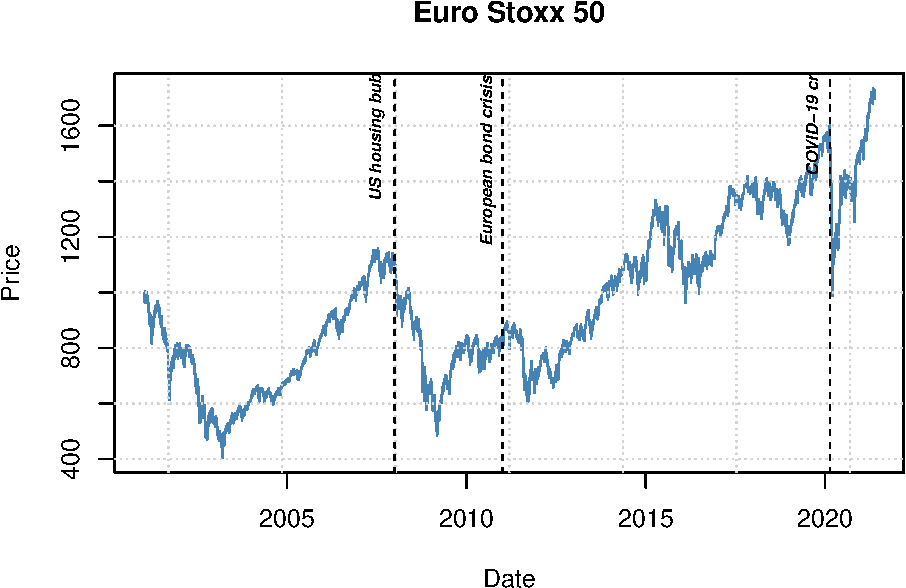
\includegraphics[width=0.75\linewidth]{_main_files/figure-latex/plot1-1} 

}

\caption{Eurostoxx 50 prices and returns}\label{fig:plot1-1}
\end{figure}
\begin{figure}

{\centering 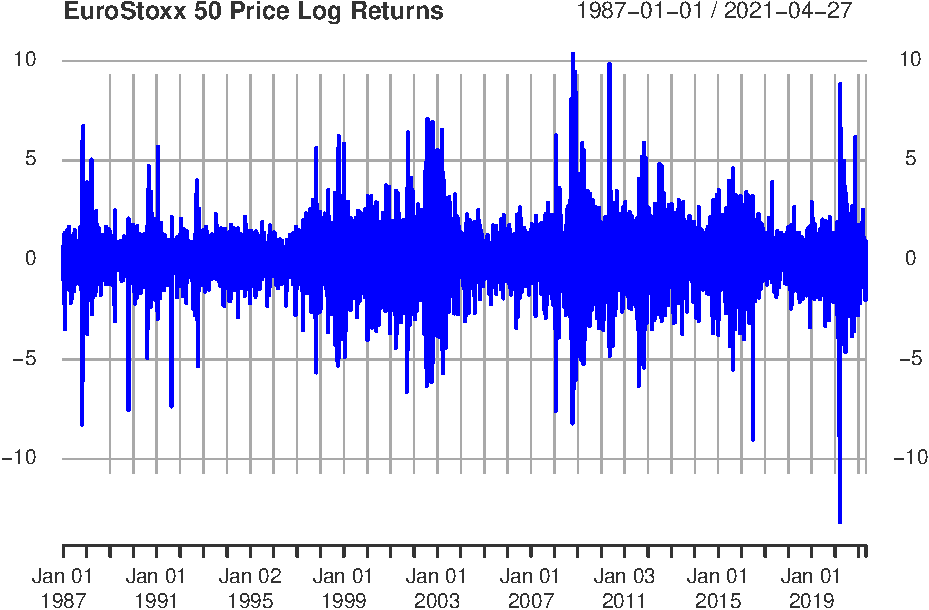
\includegraphics[width=0.75\linewidth]{_main_files/figure-latex/plot1-2} 

}

\caption{Eurostoxx 50 prices and returns}\label{fig:plot1-2}
\end{figure}
\begin{figure}

{\centering 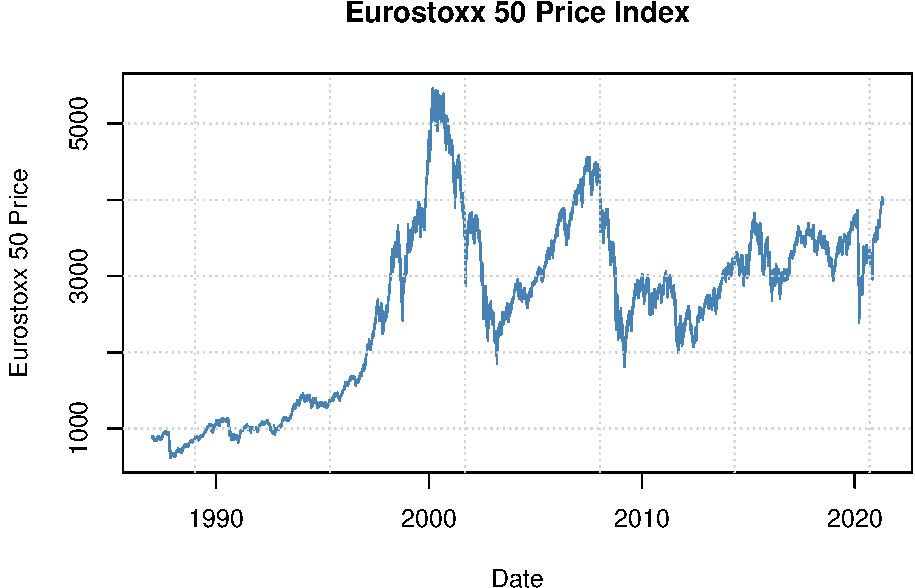
\includegraphics[width=0.75\linewidth]{_main_files/figure-latex/plot1-3} 

}

\caption{Eurostoxx 50 prices and returns}\label{fig:plot1-3}
\end{figure}

\begin{figure}

{\centering 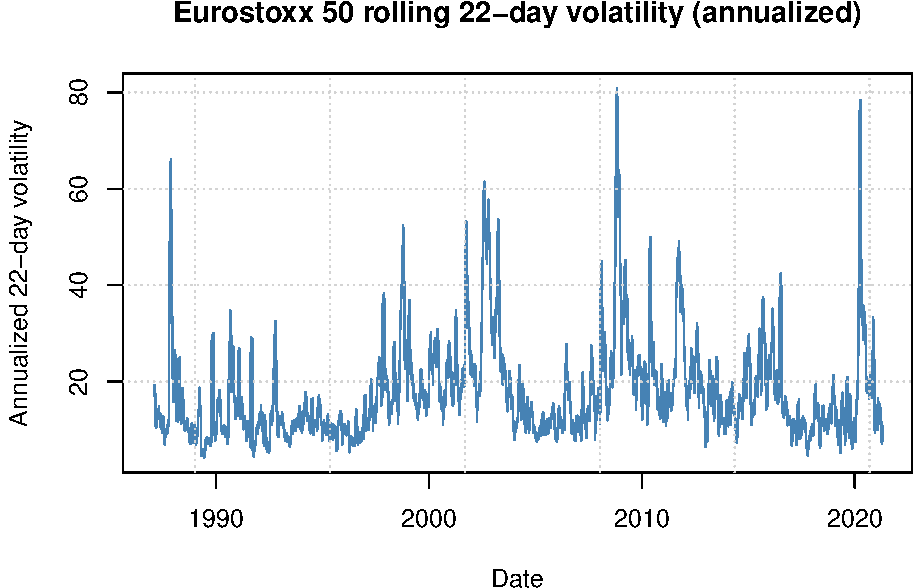
\includegraphics[width=0.75\linewidth]{_main_files/figure-latex/plot2-1} 

}

\caption{Eurostoxx 50 rolling volatility (22 days, calculated over 252 days)}\label{fig:plot2-1}
\end{figure}
\begin{figure}

{\centering 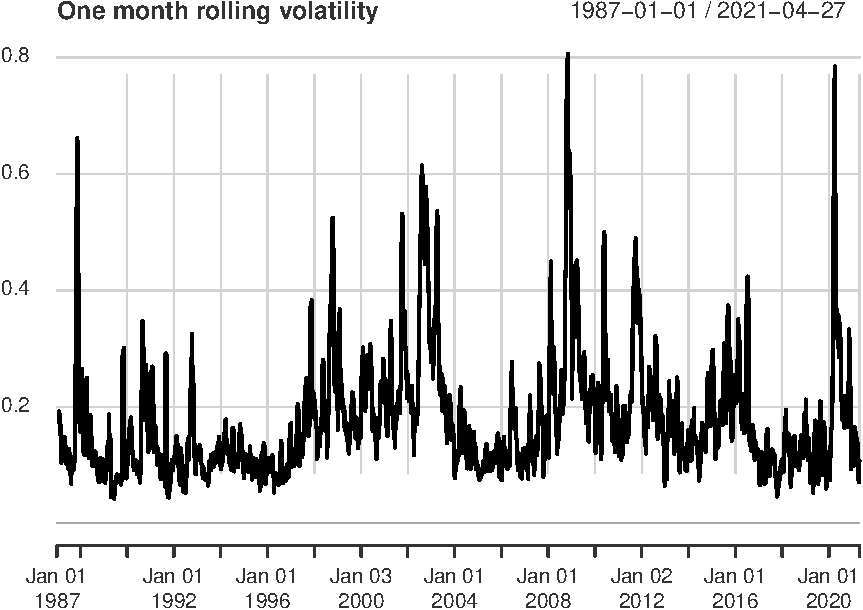
\includegraphics[width=0.75\linewidth]{_main_files/figure-latex/plot2-2} 

}

\caption{Eurostoxx 50 rolling volatility (22 days, calculated over 252 days)}\label{fig:plot2-2}
\end{figure}

\begin{figure}

{\centering 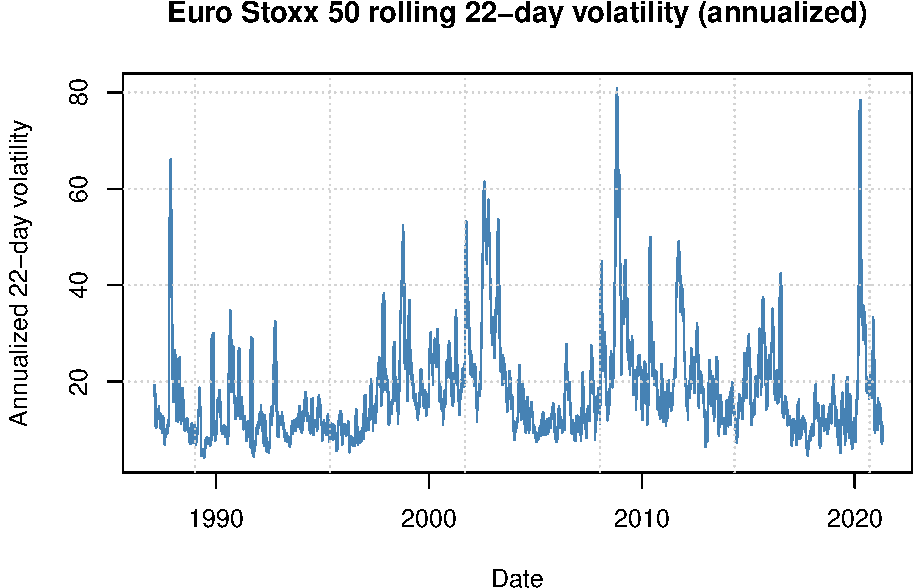
\includegraphics[width=0.75\linewidth]{_main_files/figure-latex/plot3-1} 

}

\caption{Density vs. Normal Eurostoxx 50 log returns)}\label{fig:plot3}
\end{figure}

As can be seen

\begin{figure}

{\centering 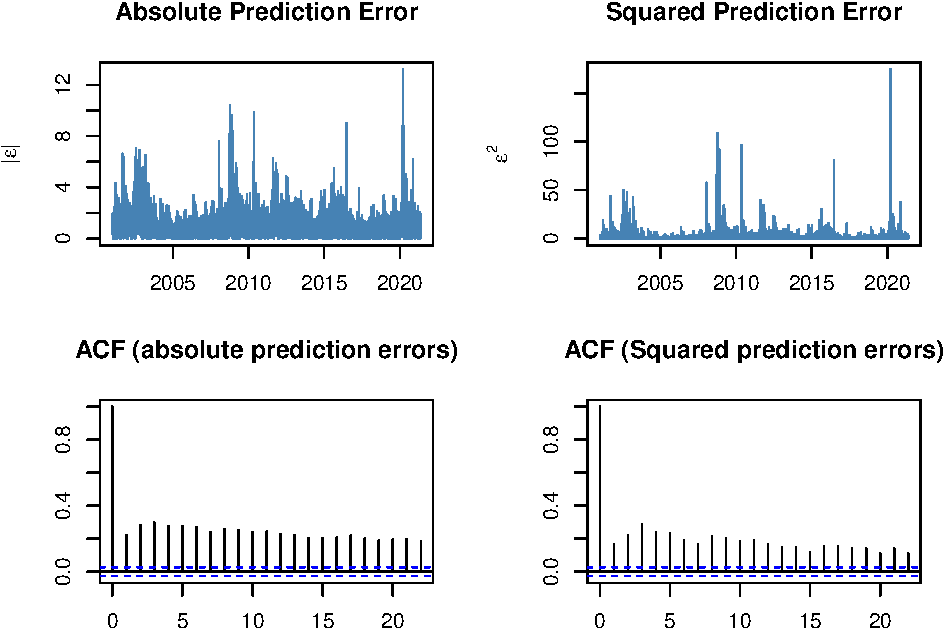
\includegraphics[width=0.75\linewidth]{_main_files/figure-latex/acfplots-1} 

}

\caption{Absolute prediction errors}\label{fig:acfplots}
\end{figure}

\newpage

\hypertarget{methodology}{%
\subsection{Methodology}\label{methodology}}

\hypertarget{garch-models}{%
\subsubsection{Garch models}\label{garch-models}}

As already mentioned in \ldots, GARCH models GARCH, EGARCH, IGARCH, GJRGARCH, NGARCH, TGARCH and NAGARCH (or TSGARCH) will be estimated. Additionally the distributions will be examined as well, including the normal, student-t distribution, skewed student-t distribution, generalized error distribution, skewed generalized error distribution and the skewed generalized t distribution.

They will be estimated using maximum likelihood. As already mentioned, fortunately, Alexios \textcite{alexios2020} has made it easy for us to implement this methodology in the R language (version 3.6.1) with the package ``rugarch'' version 1.4-4 (R univariate garch), which gives us a bit more time to focus on the results and the interpretation. Additionally

Maximum likelihood estimation is a method to find the distribution parameters that best fit the observed data, through maximization of the likelihood function, or the computationally more efficient log-likelihood function (by taking the natural logarithm). It is assumed that the return data is i.i.d. and that there is some underlying parametrized density function \(f\) with one or more parameters \(\theta\) that generates the data (\eqref{eq:pdf}). These functions are based on the joint probability distribution of the observed data (equation \eqref{eq:logl}). Subsequently, the (log)likelihood function is maximized using an optimization algorithm (equation \eqref{eq:optim}).

\begin{align} 
  y_1,y_2,...,y_N \sim i.i.d
    \\
  y_i \sim f(y|\theta)
 \label{eq:pdf}
\end{align}

\begin{align} 
 L(\theta) = \prod^N_{i=1}f(y_i|\theta)
  \\
 \log(L(\theta)) = \sum^N_{i=1} \log f(y_i |\theta)
 \label{eq:logl}
\end{align}

\begin{align} 
\theta^{*} = arg \max_{\theta} [ L] \\
\theta^{*} = arg \max_{\theta} [\log(L)]
 \label{eq:optim}
\end{align}

\begin{verbatim}
##       mean         sd 
## 0.01668214 1.30689172
\end{verbatim}

\begin{verbatim}
##       mean         sd 
## 0.01381119 0.00976596
\end{verbatim}

\begin{verbatim}
## [1] -15101.73
\end{verbatim}

\begin{verbatim}
##         df        ncp 
## 4.31096001 0.03168827
\end{verbatim}

\begin{verbatim}
##         df        ncp 
## 0.14857777 0.01100453
\end{verbatim}

\begin{verbatim}
## [1] -14149.5
\end{verbatim}

\begin{verbatim}
##       mean         sd         nu 
## 0.03160393 1.27550013 0.91274249
\end{verbatim}

\begin{verbatim}
##        mean          sd          nu 
## 0.008555584 0.015772159 0.016622605
\end{verbatim}

\begin{verbatim}
## [1] -14009.53
\end{verbatim}

\begin{verbatim}
##       mean         sd         nu         xi 
## 0.01946361 1.27515748 0.91513166 0.98174821
\end{verbatim}

\begin{verbatim}
##        mean          sd          nu          xi 
## 0.013176090 0.015786515 0.016652983 0.009638209
\end{verbatim}

\begin{verbatim}
## [1] -14008.63
\end{verbatim}

\begin{verbatim}
##      mean        sd        nu        xi 
## 0.0187729 1.4868913 2.7847974 0.9485825
\end{verbatim}

\begin{verbatim}
##       mean         sd         nu         xi 
## 0.01375064 0.05550991 0.09972285 0.01270650
\end{verbatim}

\begin{verbatim}
## [1] -13997.35
\end{verbatim}

\begin{verbatim}
## Skewed Generalized T MLE Fit
## Best Result with BFGS Maximization
## Convergence Code 0: Successful Convergence
## Iterations: NA, Log-Likelihood: -13973.01 
## 
##           Est. Std. Err.       z  P>|z|    
## mu      0.0204    0.0131  1.5574 0.1194    
## sigma   1.3214    0.0261 50.5971 0.0000 ***
## lambda -0.0397    0.0126 -3.1583 0.0016  **
## p       1.3818    0.0708 19.5077 0.0000 ***
## q       3.3093    0.5333  6.2058 0.0000 ***
## ---
## Signif. codes:  0 '***' 0.001 '**' 0.01 '*' 0.05 '.' 0.1 ' ' 1
\end{verbatim}

\begin{verbatim}
## Fitting of the distribution ' sgt ' by maximum likelihood 
## Parameters : 
##           estimate Std. Error
## mu      0.01974156 0.01263035
## sigma   1.27919321 0.01674109
## lambda -0.03189521 0.01159236
## p       1.09667765        NaN
## q       9.37999498        NaN
## Loglikelihood:  -13984.5   AIC:  27978.99   BIC:  28014.49 
## Correlation matrix:
##                 mu       sigma     lambda   p   q
## mu      1.00000000 -0.04998713 0.70347249 NaN NaN
## sigma  -0.04998713  1.00000000 0.04648083 NaN NaN
## lambda  0.70347249  0.04648083 1.00000000 NaN NaN
## p              NaN         NaN        NaN   1 NaN
## q              NaN         NaN        NaN NaN   1
\end{verbatim}

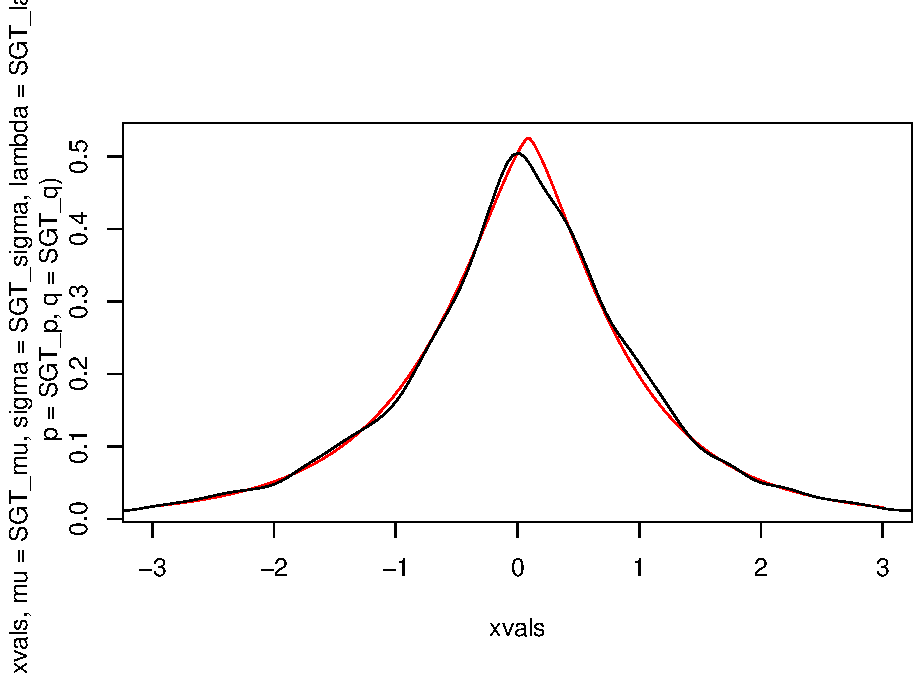
\includegraphics{_main_files/figure-latex/mlesgt-1.pdf}

\begin{verbatim}
##       mean         sd         nu         xi 
## 0.01946361 1.27515748 0.91513166 0.98174821
\end{verbatim}

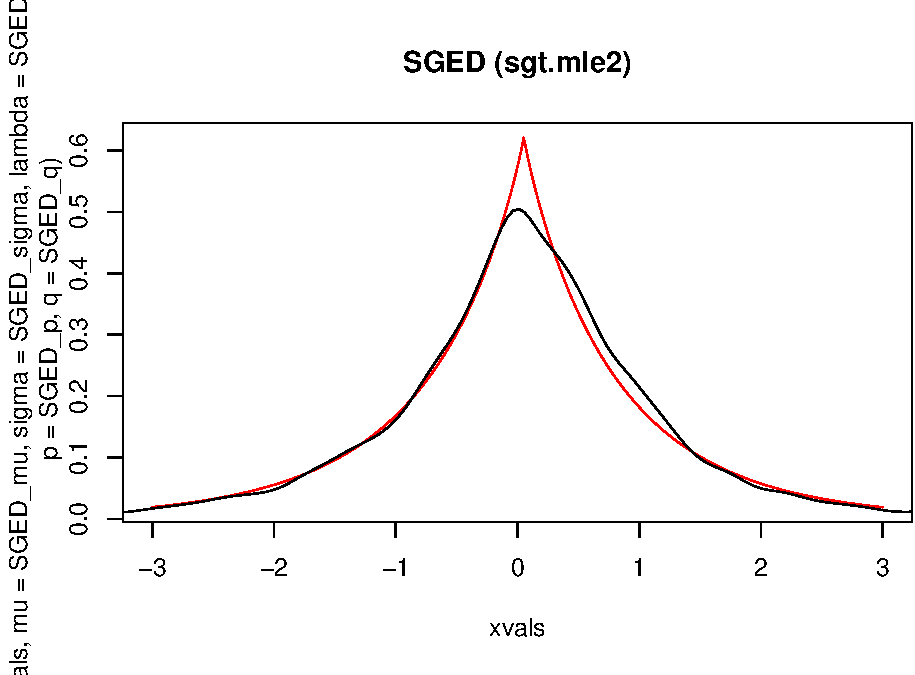
\includegraphics{_main_files/figure-latex/mlesgt-2.pdf}

\begin{verbatim}
## [1] -14008.18
\end{verbatim}

\begin{verbatim}
## [1] -14008.63
\end{verbatim}

\(A \theta + B = 0\)

\#\#\#\#Control Tests

\hypertarget{unconditional-coverage-test-of-kupiec1995}{%
\paragraph{\texorpdfstring{Unconditional coverage test of \textcite{kupiec1995} \textbackslash{}}{Unconditional coverage test of @kupiec1995 \textbackslash{}}}\label{unconditional-coverage-test-of-kupiec1995}}

A number of tests are computed to see if the value-at-risk estimations capture the actual losses well. A first one is the unconditional coverage test by \textcite{kupiec1995}. The unconditional coverage or proportion of failures method tests if the actual value-at-risk exceedances are consistent with the expected exceedances (a chosen percentile, e.g.~1\% percentile) of the VaR model. Following \textcite{kupiec1995} and \textcite{ghalanos2020}, the number of exceedence follow a binomial distribution (with thus probability equal to the significance level or expected proportion) under the null hypothesis of a correct VaR model. The test is conducted as a likelihood ratio test with statistic like in equation \eqref{eq:uccov}, with \(p\) the probability of an exceedence for a confidence level, \(N\) the sample size and \(X\) the number of exceedence. The null hypothesis states that the test statistic \(L R^{u c}\) is \(\chi^2\)-distributed with one degree of freedom or that the probability of failure \(\hat p\) is equal to the chosen percentile \(\alpha\).

\begin{align}
L R^{u c}=-2 \ln \left(\frac{(1-p)^{N-X} p^{X}}{\left(1-\frac{X}{N}\right)^{N-X}\left(\frac{X}{N}\right)^{X}}\right)
\label{eq:uccov}
\end{align}

\#\#\#\#\#Conditional coverage test of \textcite{christoffersen2001} \textbackslash{}

\textcite{christoffersen2001} proposed the conditional coverage test. It is tests for unconditional covrage and serial independence. The serial independence is important while the \(L R^{u c}\) can give a false picture while at any point in time it classifies inaccurate VaR estimates as ``acceptably accurate'' \autocite{bali2007}. For a certain VaR estimate an indicator variable, \(I_t(\alpha)\), is computed as equation \eqref{eq:ccov}.

\begin{align}
I_{t}(\alpha)=\left\{\begin{array}{ll}
1 & \text { if exceedence occurs } \\
0 & \text { if no exceedence occurs }
\end{array} .\right.
\label{eq:ccov}
\end{align}

It involves a likelihood ratio test's null hypothesis is that the statistic is \(\chi^2\)-distributed with two degrees of freedom or that the probability of violation \(\hat p\) (unconditional coverage) as well as the conditional coverage (independence) is equal to the chosen percentile \(\alpha\).

\hypertarget{dynamic-quantile-test}{%
\paragraph{Dynamic quantile test \textbackslash{}}\label{dynamic-quantile-test}}

\textcite{engle2004} with the aim to provide completeness to the conditional coverage test of \textcite{christoffersen2001} developed the Dynamic quantile test. It consists in testing some restriction in a

\clearpage

\hypertarget{analysis}{%
\chapter{Empirical Findings}\label{analysis}}

\minitoc 

\hypertarget{results-of-garch-with-constant-higher-moments}{%
\section{Results of GARCH with constant higher moments}\label{results-of-garch-with-constant-higher-moments}}

\hypertarget{results-of-garch-with-time-varying-higher-moments}{%
\section{Results of GARCH with time-varying higher moments}\label{results-of-garch-with-time-varying-higher-moments}}

\begin{figure}

{\centering 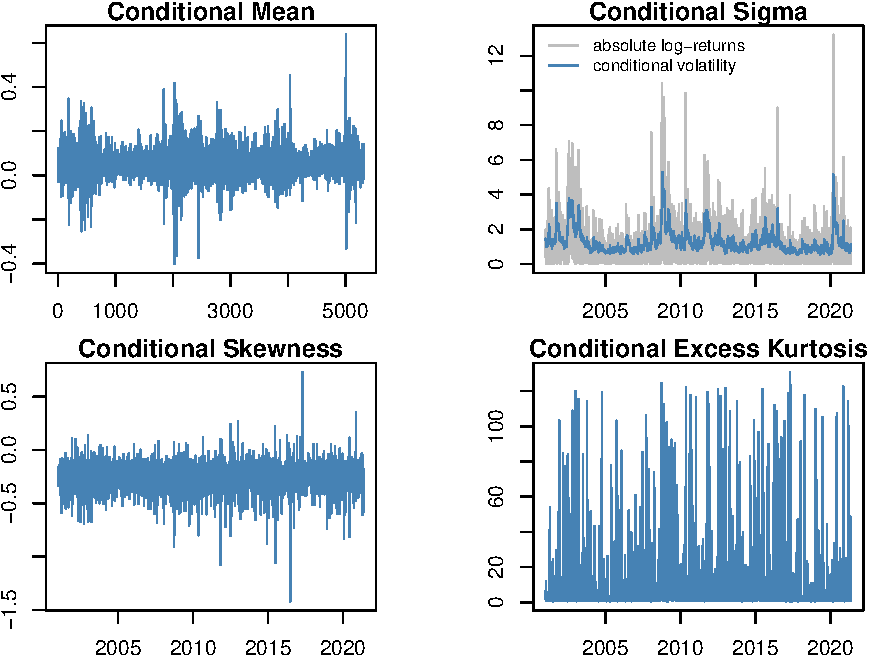
\includegraphics{_main_files/figure-latex/figureACDmoments-1} 

}

\caption{Dynamics of the ACD model}\label{fig:figureACDmoments}
\end{figure}

\hypertarget{robustness-analysis}{%
\chapter{Robustness Analysis}\label{robustness-analysis}}

\minitoc 

\hypertarget{specification-checks}{%
\section{Specification checks}\label{specification-checks}}

In order to check if the models are specified correctly, some specification checks have to be performed. The specification checks have to be done on the standardized residuals of the estimated GARCH model given by the following equation:
\[ 
\hat{Z_t} = \dfrac{\hat{\varepsilon_t}}{\hat{\sigma_t}} = \dfrac{R_t - \hat{\mu}}{\hat{\sigma_t}}
\]
\#\#\# Residual heteroscedasticity
Ljung-Box test on the squared or absolute standardized residuals.

\hypertarget{eye-balling-econometrics}{%
\subsection{Eye-balling econometrics}\label{eye-balling-econometrics}}

Autocorrelation function of the standardized residuals and autocorrelation function of the squared standardized residuals.

Then the density can be examined standardized residuals and compared with the normal distribution.

Also the QQ-plot can be examined.

\hypertarget{gmm-test}{%
\subsection{GMM test}\label{gmm-test}}

zero-mean
unit-variance
not skewed
no excess kurtosis
no serial correlation in the squares
no serial correlation in the cubes
no serial correlation in the squares

\hypertarget{conclusion}{%
\chapter*{Conclusion}\label{conclusion}}
\addcontentsline{toc}{chapter}{Conclusion}

\startappendices

\hypertarget{appendix}{%
\chapter{Appendix}\label{appendix}}


%%%%% REFERENCES

% JEM: Quote for the top of references (just like a chapter quote if you're using them).  Comment to skip.
% \begin{savequote}[8cm]
% The first kind of intellectual and artistic personality belongs to the hedgehogs, the second to the foxes \dots
%   \qauthor{--- Sir Isaiah Berlin \cite{berlin_hedgehog_2013}}
% \end{savequote}

\setlength{\baselineskip}{0pt} % JEM: Single-space References

{\renewcommand*\MakeUppercase[1]{#1}%
\printbibliography[heading=bibintoc,title={\bibtitle}]}


\end{document}
